%%
%% This is file `sample-xelatex.tex',
%% generated with the docstrip utility.
%%
%% The original source files were:
%%
%% samples.dtx  (with options: `sigconf')
%% 
%% IMPORTANT NOTICE:
%% 
%% For the copyright see the source file.
%% 
%% Any modified versions of this file must be renamed
%% with new filenames distinct from sample-xelatex.tex.
%% 
%% For distribution of the original source see the terms
%% for copying and modification in the file samples.dtx.
%% 
%% This generated file may be distributed as long as the
%% original source files, as listed above, are part of the
%% same distribution. (The sources need not necessarily be
%% in the same archive or directory.)
%%

\documentclass[sigconf, nonacm]{acmart}

\usepackage{mwe}
\usepackage[colorinlistoftodos,prependcaption,textsize=tiny]{todonotes}


%%
%% \BibTeX command to typeset BibTeX logo in the docs
\AtBeginDocument{%
  \providecommand\BibTeX{{%
    \normalfont B\kern-0.5em{\scshape i\kern-0.25em b}\kern-0.8em\TeX}}}

\begin{document}

%%
%% The "title" command has an optional parameter,
%% allowing the author to define a "short title" to be used in page headers.
\title{Express Data Queueing}

%%
%% The "author" command and its associated commands are used to define
%% the authors and their affiliations.
%% Of note is the shared affiliation of the first two authors, and the
%% "authornote" and "authornotemark" commands
%% used to denote shared contribution to the research.
\author{Freysteinn Alfreðsson}
\email{freysteinn.alfredsson@kau.se}
\orcid{0000-0003-1516-9370}
\affiliation{%
  \institution{Department of Computer Science}
  \city{Karlstad}
  \country{Sweden}
}
\author{Per Hurtig}
\email{per.hurtig@kau.se}
\affiliation{%
  \institution{Department of Computer Science}
  \city{Karlstad}
  \country{Sweden}
}
%%\orcid{0000-0003-1516-9370}
\author{Anna Brunstrom}
\email{anna.brunstrom@kau.se}
\affiliation{%
  \institution{Department of Computer Science}
  \city{Karlstad}
  \country{Sweden}
}

\author{Toke Høiland-Jørgensen}
\email{toke@redhat.com}
\affiliation{%
  \institution{Red hat}
  \country{Denmark}
}

\author{Jesper Dangaard Brouer}
\email{brouer@redhat.com}
\affiliation{%
  \institution{Red hat}
  \country{Denmark}
}

%%
%% By default, the full list of authors will be used in the page
%% headers. Often, this list is too long, and will overlap
%% other information printed in the page headers. This command allows
%% the author to define a more concise list
%% of authors' names for this purpose.
\renewcommand{\shortauthors}{Alfreðsson, et al.}

\begin{abstract}
\end{abstract}

%%
%% Keywords. The author(s) should pick words that accurately describe
%% the work being presented. Separate the keywords with commas.
\keywords{XDP, BPF, BPF, Queueing, Linux, Scheduling}

%%
%% This command processes the author and affiliation and title
%% information and builds the first part of the formatted document.
\maketitle

\section{Introduction}

The Linux kernel is a widely used platform in devices that range from IoT devices, cellphones, home and enterprise routers to servers and cloud offerings. One of the revolutionary technologies of the Linux kernel is the BPF framework, which has changed the way we extend the kernel. This framework is an in-kernel runtime environment that allows domain-specific code to execute within the kernel safely using predefined hooks. One such hook is the Linux eXpress Data Path\cite{hoiland2018express}, or XDP, which has found numerous uses in the industry, such as DoS attack mitigation, load-balancers, and intrusion prevention systems.

XDP provides a high-performance programmable network data path and allows programmers to process packets early out of the driver. While XDP excels in forwarding packets, it currently has no mechanism for queuing or reordering of packets and cannot implement traffic scheduling policies. Packet scheduling is a common task on network equipment, and like for other aspects of networking, there is a growing interest for bringing programmability to this domain. For the Linux kernel, making packet scheduling fully programmable through BPF is the obvious answer to this trend.

This paper presents our work on adding programmable packet scheduling to XDP, which we also provide as a Qdisc. We have designed a programmable packet scheduling framework in BPF using recently proposed schemes for programmable queues. This extension allows programmers to define their packet schedulers using BPF while benefiting from the XDP fast data path.


\section{Packet Scheduling, Traffic Shaping, and Queue Management}

Packet schedulers are an essential and integral part of today's networks. They provide the means of controlling the policy and quality requirements within a network for customers and services. However, at its core, the primary function of the packet scheduler is to arrange or rearrange packets to meet the requirements of the network. Most of these requirements are to improve the latency of specific flows or to improve fairness between flows. For instance, video streaming services would like to ensure that clients get fair access to their video streams. Moreover, a service provider might want to prioritize traffic of their productions servers over their testing servers. Therefore, having the flexibility to adapt the packet scheduling algorithm to the requirements of the network in question can significantly improve its overall quality.


\begin{figure}
  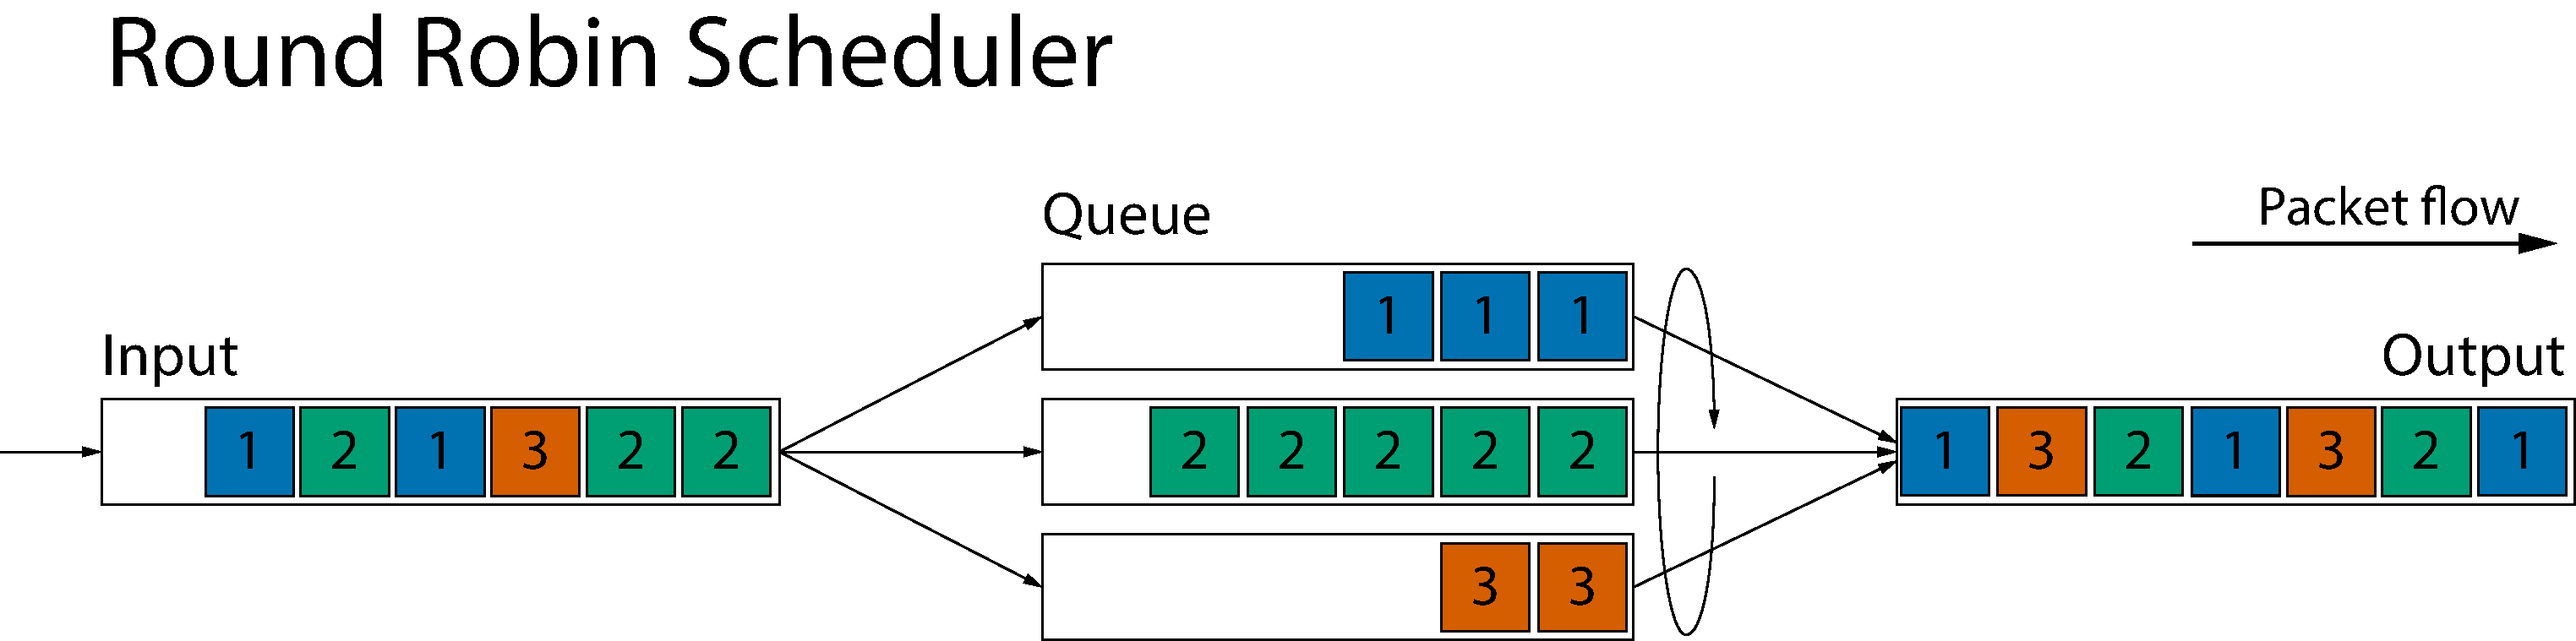
\includegraphics[width=\linewidth]{round-robin.pdf}
  \caption{\label{fig:round_robin}}
\end{figure}

A simple example of a packet scheduler is the round-robin scheduler\cite{nagle1987packet}, depicted in Figure~\ref{fig:round_robin}. This scheduler sorts the incoming packets by flow into different queues, which it then dequeues from in a round-robin fashion, or by taking one packet from each queue at the time. This simple scheduler can provide proportional queue fairness between flows to improve the packet latency of low throughput flows.

\begin{figure}
  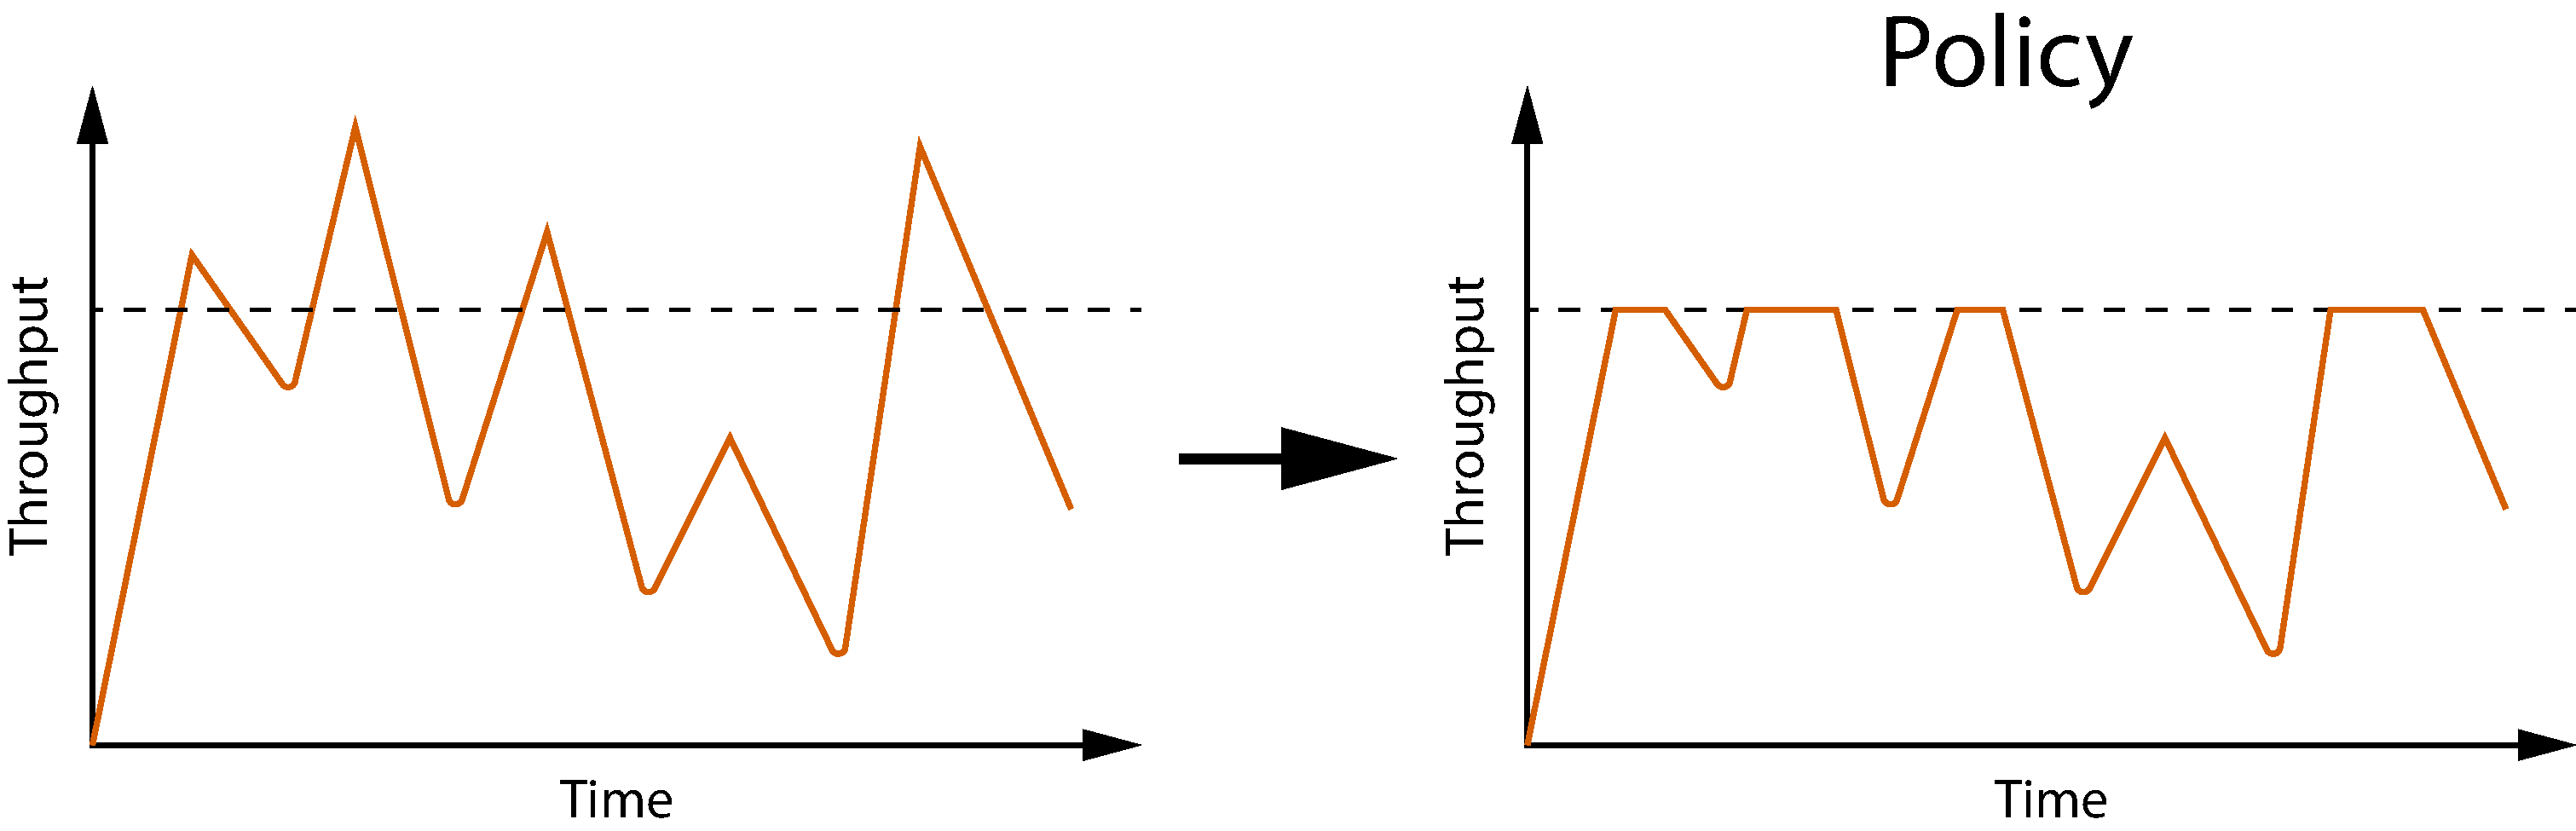
\includegraphics[width=\linewidth]{traffic-policy.pdf}
  \caption{\label{fig:traffic_policy}}
\end{figure}

\begin{figure}
  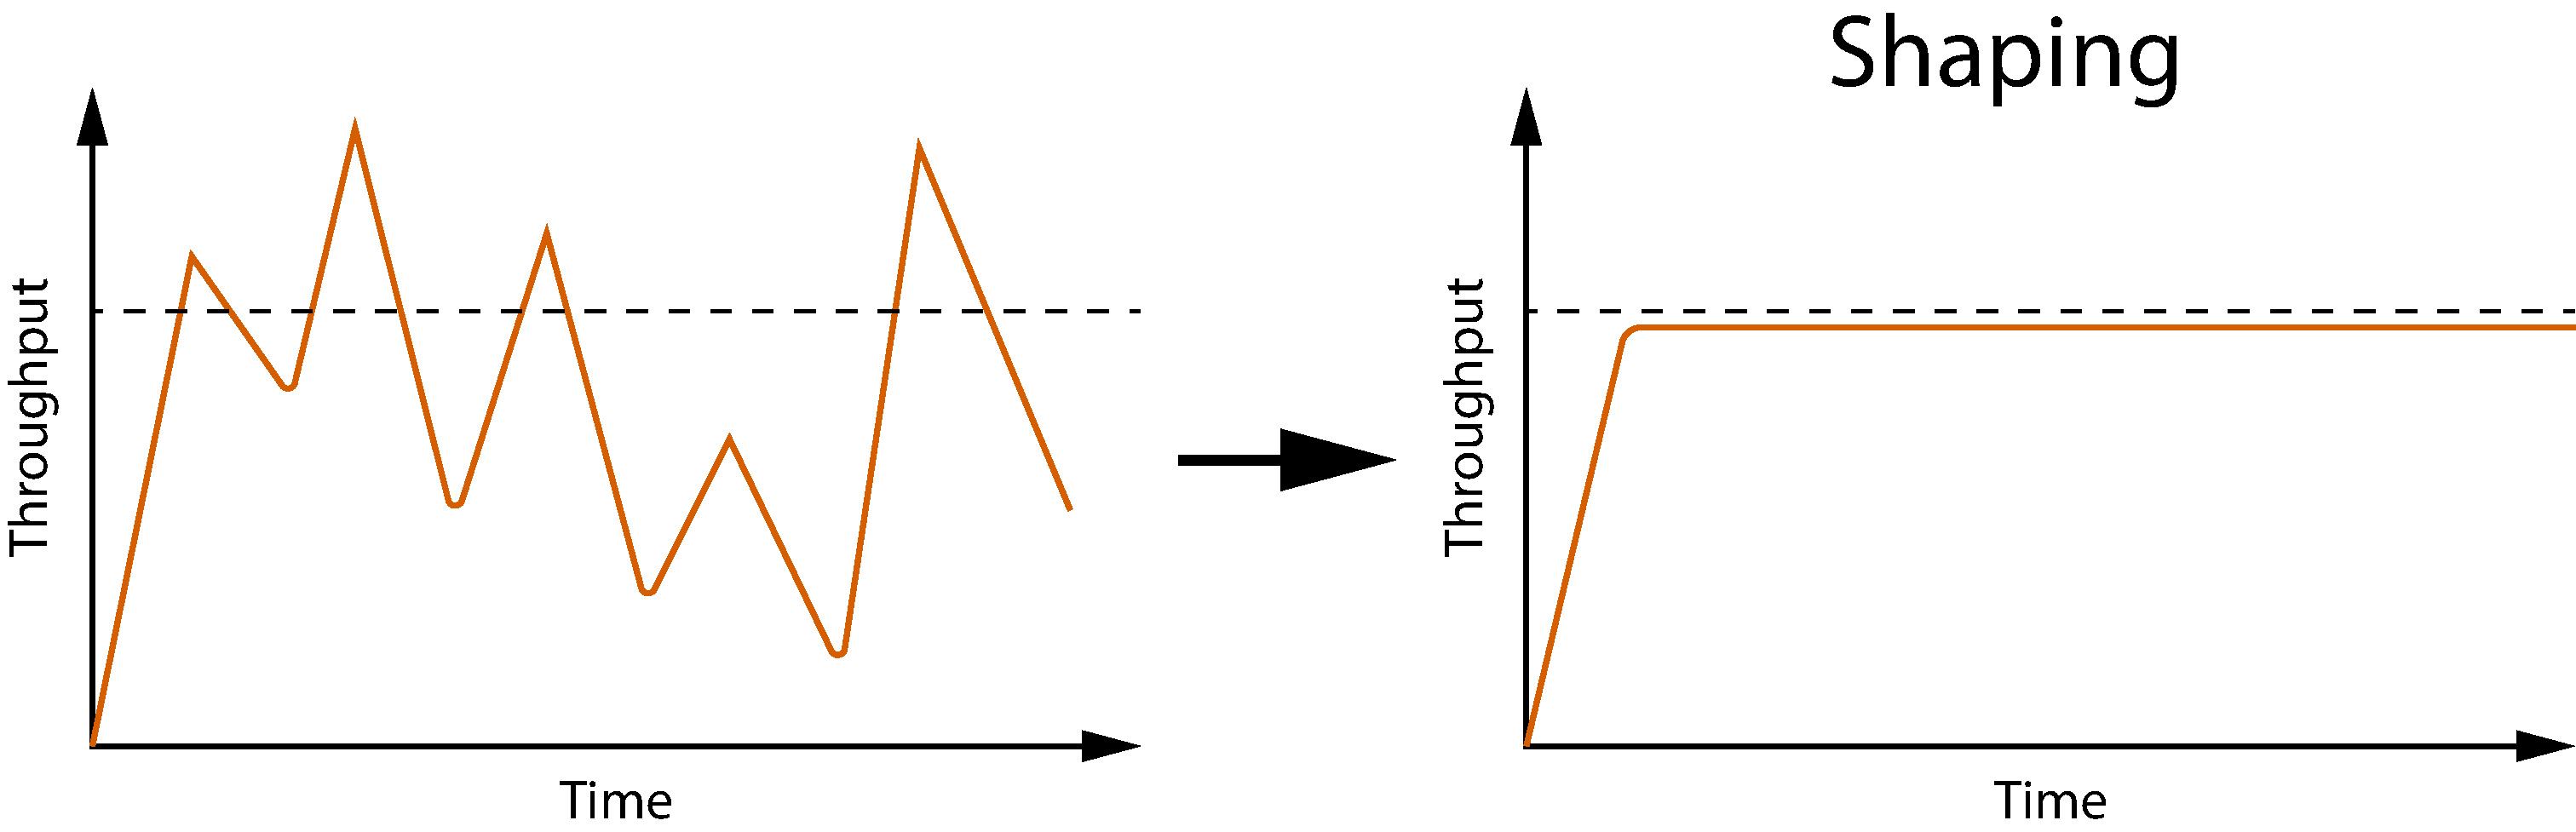
\includegraphics[width=\linewidth]{traffic-shaping.pdf}
  \caption{\label{fig:traffic_shaping}}
\end{figure}


Another crucial component related to packet schedulers is the capability of delaying packets. This capability allows packet scheduling algorithms to provide traffic shaping, as seen in figure \ref{fig:traffic_shaping}. These algorithms are referred to as non-work conserving algorithms because they do not necessarily use the total capacity of the network interface, while work-conserving algorithms never delay packets and can use their total capacity. The non-work conserving capability can restrict a service from dominating the traffic and ensure that high-priority event packets are not delayed by always leaving enough room in the queues to squeeze them in without compromising the guaranteed predictability of the shaped traffic.

Queue management is also another essential topic related to packet schedulers and is the art of controlling how many packets the queues can queue. A significant problem in today's environments is buffer bloat, where buffers favor large buffers for throughput by sacrificing latency. Buffer bloat can negatively affect low latency applications such as video conferencing, online gaming, and other interactive applications. Therefore, queue management is an integral part of the queueing process, while it is not usually considered part of the packet scheduling algorithm.


\section{Linux Kernel Networking Subsystem}

\begin{figure}
  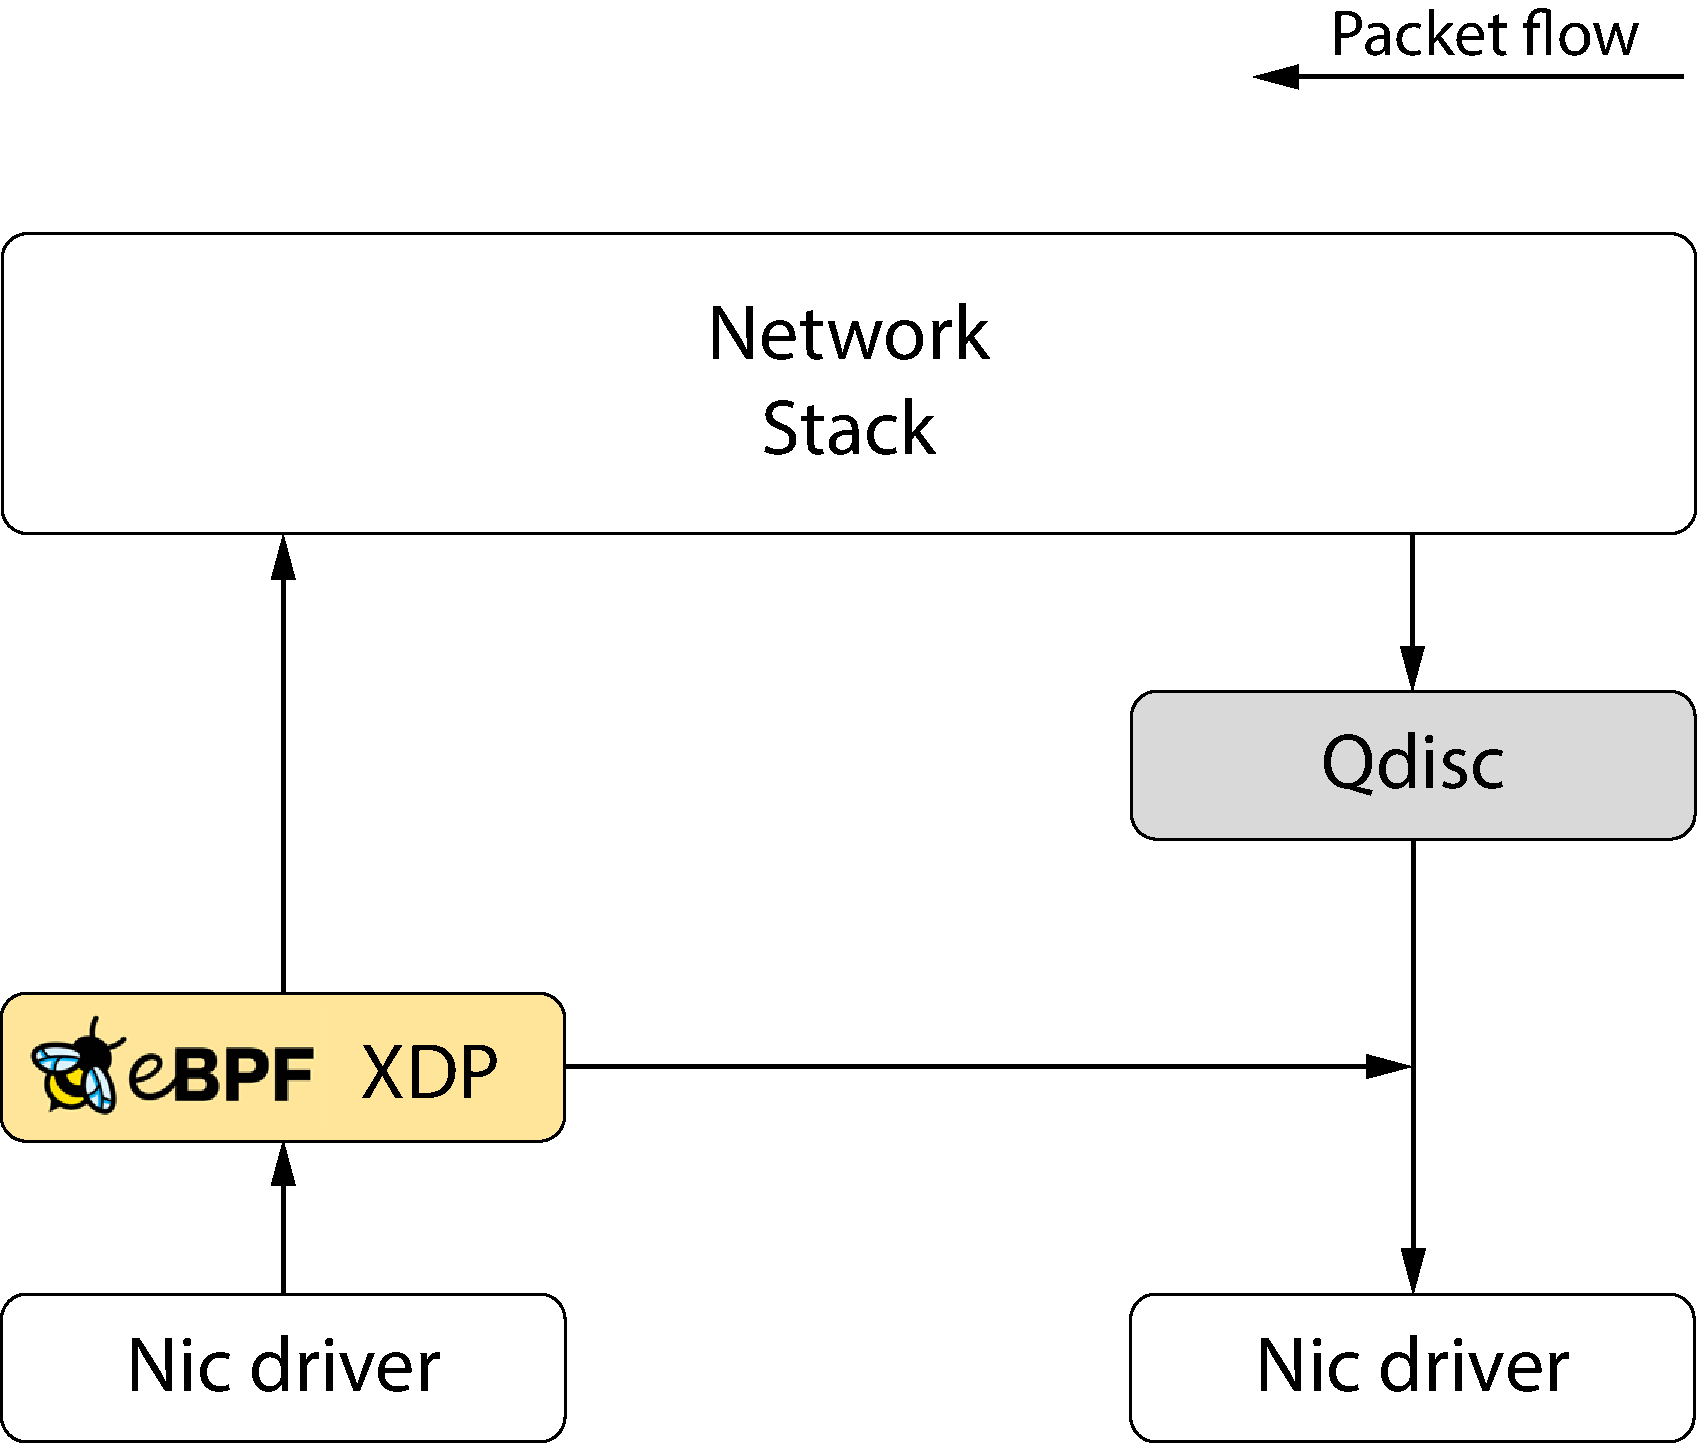
\includegraphics[width=\linewidth]{network-overview.pdf}
  \caption{\label{fig:network_overview}}
\end{figure}

The Linux kernel Networking stack is highly mature and a flexible piece of software. It contains a hardware abstraction layer, a traffic control layer responsible for routing and firewall rules, and layers responsible for handling the TCP/IP networking layers. Part of the traffic control layer is the Queueing discipline layer or the Qdisc layer for short. This layer gives the Linux kernel flexible packet scheduling capabilities and an interface to create new packet schedulers as loadable kernel modules. However, due to the immense speed increases in modern network devices, the kernel's networking stack has become a bottleneck. This obstacle has prompted network vendors and researchers to create alternative solutions to mitigate this performance bottleneck. One such solution is DPDK which bypasses the Linux kernel and communicates directly to the networking hardware. An alternative solution to bypassing the Linux kernel is XDP, which creates a fast data path within the Linux kernel while retaining the kernel and user-space separation. We provide a simplified diagram of the Linux kernel's networking infrastructure in Figure \ref{fig:network_overview} which shows the relevant parts related to our work in this paper.

The leading networking data structure in the Linux kernel is the sk\_buff. The sk\_buff is a large data structure with multiple fields related to all layers in the network stack and gets populated through each layer of the network stack, including the Qdisc layer. However, XDP handles network packets in the driver right after a DMA synchronization. Therefore, it does not use the sk\_buff data structure but represents the packet using a slimmer data structure called xdp\_mp, which does not get converted into a sk\_buff unless the XDP hook passes the packet onto the network stack.



\subsection{The Linux Kernel Packet Queueing Discipline (Qdisc)}

Packet scheduling in the Linux kernel is handled by the Qdisc subsystem. It is a mature system that is capable of wast operations, such as policing, shaping, classifying, dropping, and marking traffic.

\begin{itemize}
  \item Explain where in the network pipe the Qdiscs are located.
  \item Explain that the Qdisc layer allows us to create hierarchies of preexisting Qdiscs.
  \item Explain what the Qdisc classifier does.
  \item Explain what the BPF Qdisc classifier does and why it does not fulfill our needs.
\end{itemize}


%\section{Packet Schedulers in Practice}
%
%\todo[inline]{Frey: This section needs a new name. The idea with this section is to explain why we care about this work and what the requirements are.}
%
%\begin{itemize}
%  \item Explain what is not possible using today's packet schedulers.
%  \item Explain why you would like to be able to schedule traffic
%\end{itemize}


\section{Programmable Packet Schedulers}

\begin{figure}
  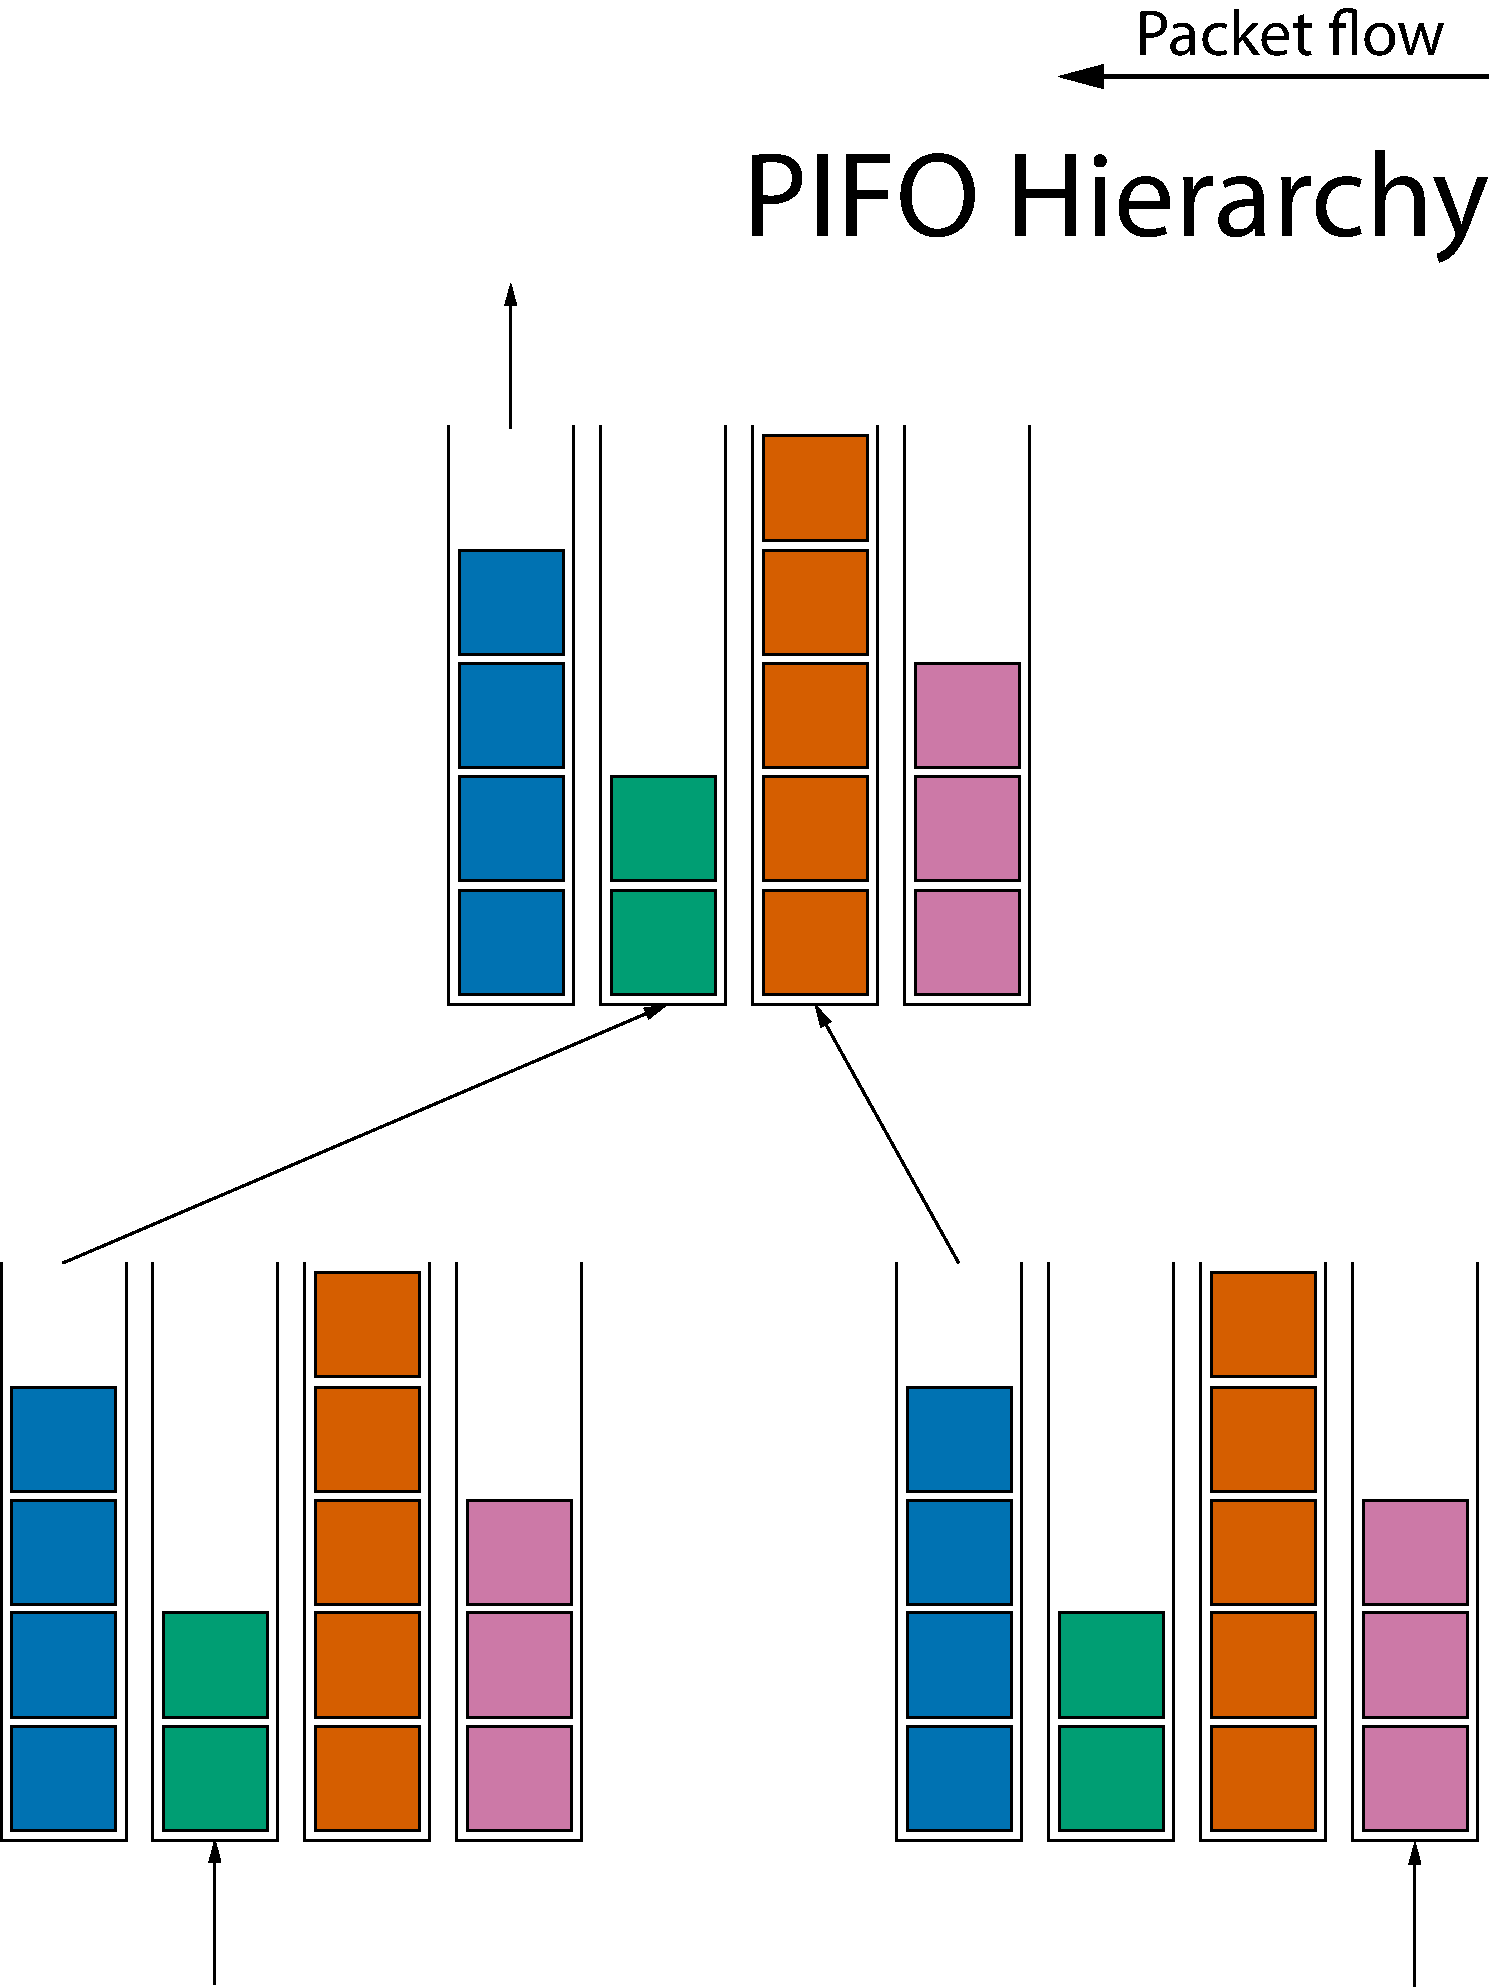
\includegraphics[width=0.3\linewidth]{pifo-hierarchy.pdf}
  \caption{\label{fig:pifo_hierarchy}}
\end{figure}

Traditionally, network equipment and operating systems provide a handful of packet scheduling algorithms. This limited number of schedulers forced companies to tune the parameters of these algorithms to meet their requirements. However, modern networking equipment has started to provide programmable network capabilities, which the network engineer can leverage using specialized programming languages such as P4\cite{p4} or standard programming languages such as C, such as in the case of traditional operating systems. This new paradigm shift allows the network designers to create custom logic and custom packet scheduling solutions optimized for their specific unique use case. Therefore, instead of tuning the network to the limitations of the packet scheduling algorithm, they can tune their packet scheduling algorithm directly to their network requirements.

Consequently, the building blocks of a programmable packet scheduling framework need to be straightforward, fast, and easy to understand. Therefore, the essential part of creating a programmable packet scheduling framework is to provide a flexible data structure. Hence, a hot research topic has been to develop a flexible data structure that programmers can leverage to implement their packet schedulers. However, due to the vast speeds of modern network interfaces, severe limitations are put on these data structures. These limitations differ depending on if the data structure is hardware or software-based. However, they all share common traits, such as algorithms queueing packets into the data structure based on a ranking function directed by a scheduling policy and periodically dequeued according to the scheduled packet order. They also share that the data structures are simple and allow flexibility by creating hierarchies of the data structures, as seen in Figure~\ref{fig:pifo_hierarchy}. However, they differ on if they allow internal reordering on enqueue or reordering on dequeue. They also differ in their scheduling granularity. Most simple data structures schedule individual packets, while more complex data structures allow scheduling flows.

Hardware-based scheduling data structures limit the amount of complexity and the physical size these data structures can take due to cost and efficiency. Therefore, researchers have created simple data structures, such as the Push-In First-Out, described in section~\ref{sec:pifo} which are easy to implement in hardware but do impose limits that we can circumvent in software.

On the other hand, software-based scheduling data structures have severe limitations due to the time constraint needed to keep up with line-rate, despite the growing capabilities of CPUs. The number of instructions we can use per packet excludes complex data structures such as red-black trees or complicated heap algorithms. Therefore, some data structures, such as Eiffel\cite{Saeed2019} propose a data structure with specific software-specific optimizations.


\subsection{PIFO and SP-PIFO\label{sec:pifo}}

Despite its simplicity, the Push-In First-Out data structure\cite{Sivaraman2016} is quite versatile and allows the programmer to implement a wide range of packet schedulers. From a programmer's perspective, the programmer only needs to decide what order to schedule packets and when to schedule them for non-work conserving algorithms. However, one limitation of the PIFO is that it is a set of queues for each possible rank. Therefore, the more granularity of ranks, the more resources the PIFO needs. This limitation limits how large the PIFO can be both in hardware and software implementations. A mitigation to this limitation is the SP-PIFO\cite{Alcoz2020}, which approximates a large PIFO using a smaller PIFO.

\begin{figure}
  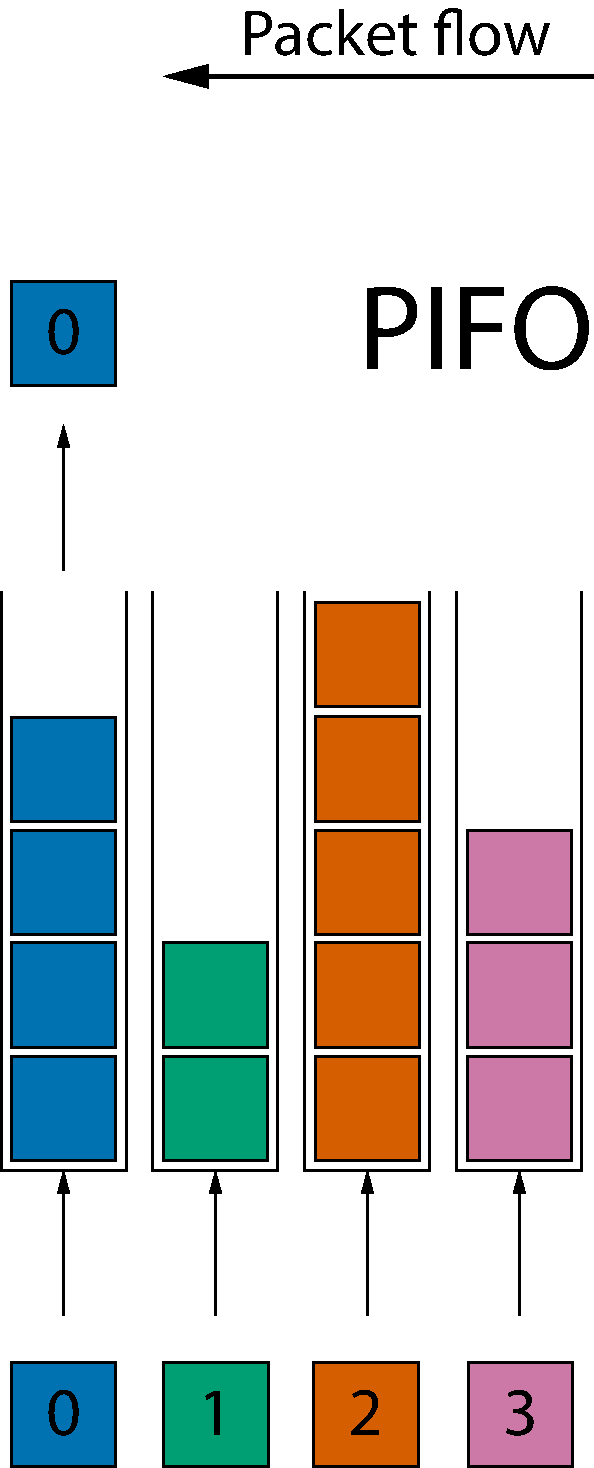
\includegraphics[width=0.25\linewidth]{pifo.pdf}
  \caption{\label{fig:pifo}}
\end{figure}

\subsubsection{Data Structure}

The PIFO is a set of queues that the programmer can push packets into depending on their rank, as shown in Figure~\ref{fig:pifo}. However, the programmer can only dequeue from the head of the PIFO. The programmer can only order packets on enqueue to the queues, but the PIFO does not allow reordering the packets within a queue, nor on deqeue. This limitation does exclude the PIFO from implementing some packet scheduling algorithms, such as pFabric\cite{alizadeh2013pfabric}.


\subsection{Eiffel}

The Eiffel data structure is a PIFO with a couple of alterations. First, in Eiffel, the programmer can schedule flows or packets, depending on the algorithm. Second, the programmer can do on-dequeue scheduling, where incoming and outgoing packets belonging to a specific flow can change the rank of all packets of the flow on both enqueue and dequeue due to per-flow scheduling.
Also, because the Eiffel data structure is a software implementation, the Eiffel paper proposes a few software-based optimizations to improve the performance of the Eiffel. One such optimization is to use a bit-field to keep track of queues containing packets and use the CPUs Find-First-Set instruction to accelerate the lookup in the bit lookup table. The lookup table can be further segmented into a tree-based lookup table when the Eiffel has many ranks.


\subsection{Calendar-queues}

\begin{itemize}
  \item Explain that it supports both work and non-work conserving scheduling.
\end{itemize}


\subsubsection{Data Structure}

\begin{itemize}
  \item Explain that it uses a circular buffer with a hand like an analog clock. The slots represent when the scheduler will dequeue in the future. While the hand points to the packets that are dequeing.
\end{itemize}


\section{The BPF framework}

The BPF framework is an in-kernel runtime environment that allows specialized programs to execute in the kernel safely. These programs attach themselves to hooks provided by the different subsystems of the kernel. These hooks limit what the programs can do and define what type of BPF programs can exist. These types of programs vary but predominantly, they are related to networking, tracing, and security. At its core, BPF is an instruction set. However, as a framework, it provides a key-value store that enables inter-process communication called BPF maps, in-kernel helper functions, and toolchains to create and manage BPF programs from user-space.

\todo[inline]{Frey: Because we all know what BPF is, I am going to collapse these BPF sections and make it shorter and simpler.}

\begin{itemize}
  \item Explain BPF maps and their scope.
  \item Explain what hooks are and that BPF allows helper functions.
  \item Explain how BPF programs are loaded using the bpf system call.
\end{itemize}


\subsection{Instruction-set}

\todo[inline]{Frey: I think I will remove this section either completely, or at least remove the extra details.}

The BPF instruction set is 64-bit and consists of eleven registers listed in table ~\ref{table:BPF_registers}. It contains a little over a hundred instructions. However, the current format defines the opcode as the first octet of the instruction. Therefore, in the current design, it could only support 256 instructions. The currently available instructions are limited to Arithmetic Logic Unit (ALU) instructions, byte-swap instructions for Endian handling, memory, and branch instructions.

\begin{table}
  \caption{Frequency of Special Characters}
  \label{table:BPF_registers}
  \begin{tabular}{ll}
    \toprule
    Register & Type                    \\
    \midrule
    R0       & Return value            \\
    R1-R5    & Parameters to functions \\
    R6-R9    & Callee saved registers  \\
    R10      & Read-only stack pointer \\
    \bottomrule
\end{tabular}
\end{table}


\subsection{Express Data Path (XDP)}

XDP\cite{hoiland2018express} is a type of BPF program that is attached directly to the RX path of a network interface to allow the programmer direct manipulation of packets from the network driver. Its primary use cases are high-performance packet processing and the ability to bypass the kernel's network stack by redirecting the packet to different locations, such as back out the same device, to another device, or dropping the packet entirely. XDP also provides helper functions that allow the programmer to call particular parts of the network stack, such as fib lookups.

While XDP excels at forwarding packets, it does not support packet reordering or packet scheduling. Our objective in this paper is to extend XDP to support packet scheduling. This support includes adding helper functions and extra hooks for dequeuing and pacing operations.


\subsection{BPF Qdisc Classifiers}

Currently, the Qdisc layer only has a BPF classifier capable of manipulating packets and directing them into excising Qdiscs that are not programmable using BPF. While this does provide a form of programable packet scheduling, it relies exclusively on the Qdisc layer, which XDP can not use. We aim to provide a BPF based packet scheduling framework for XDP and as a standalone Qdisc.


\section{A Programmable Packet Scheduling Framework in BPF}

\begin{figure}

  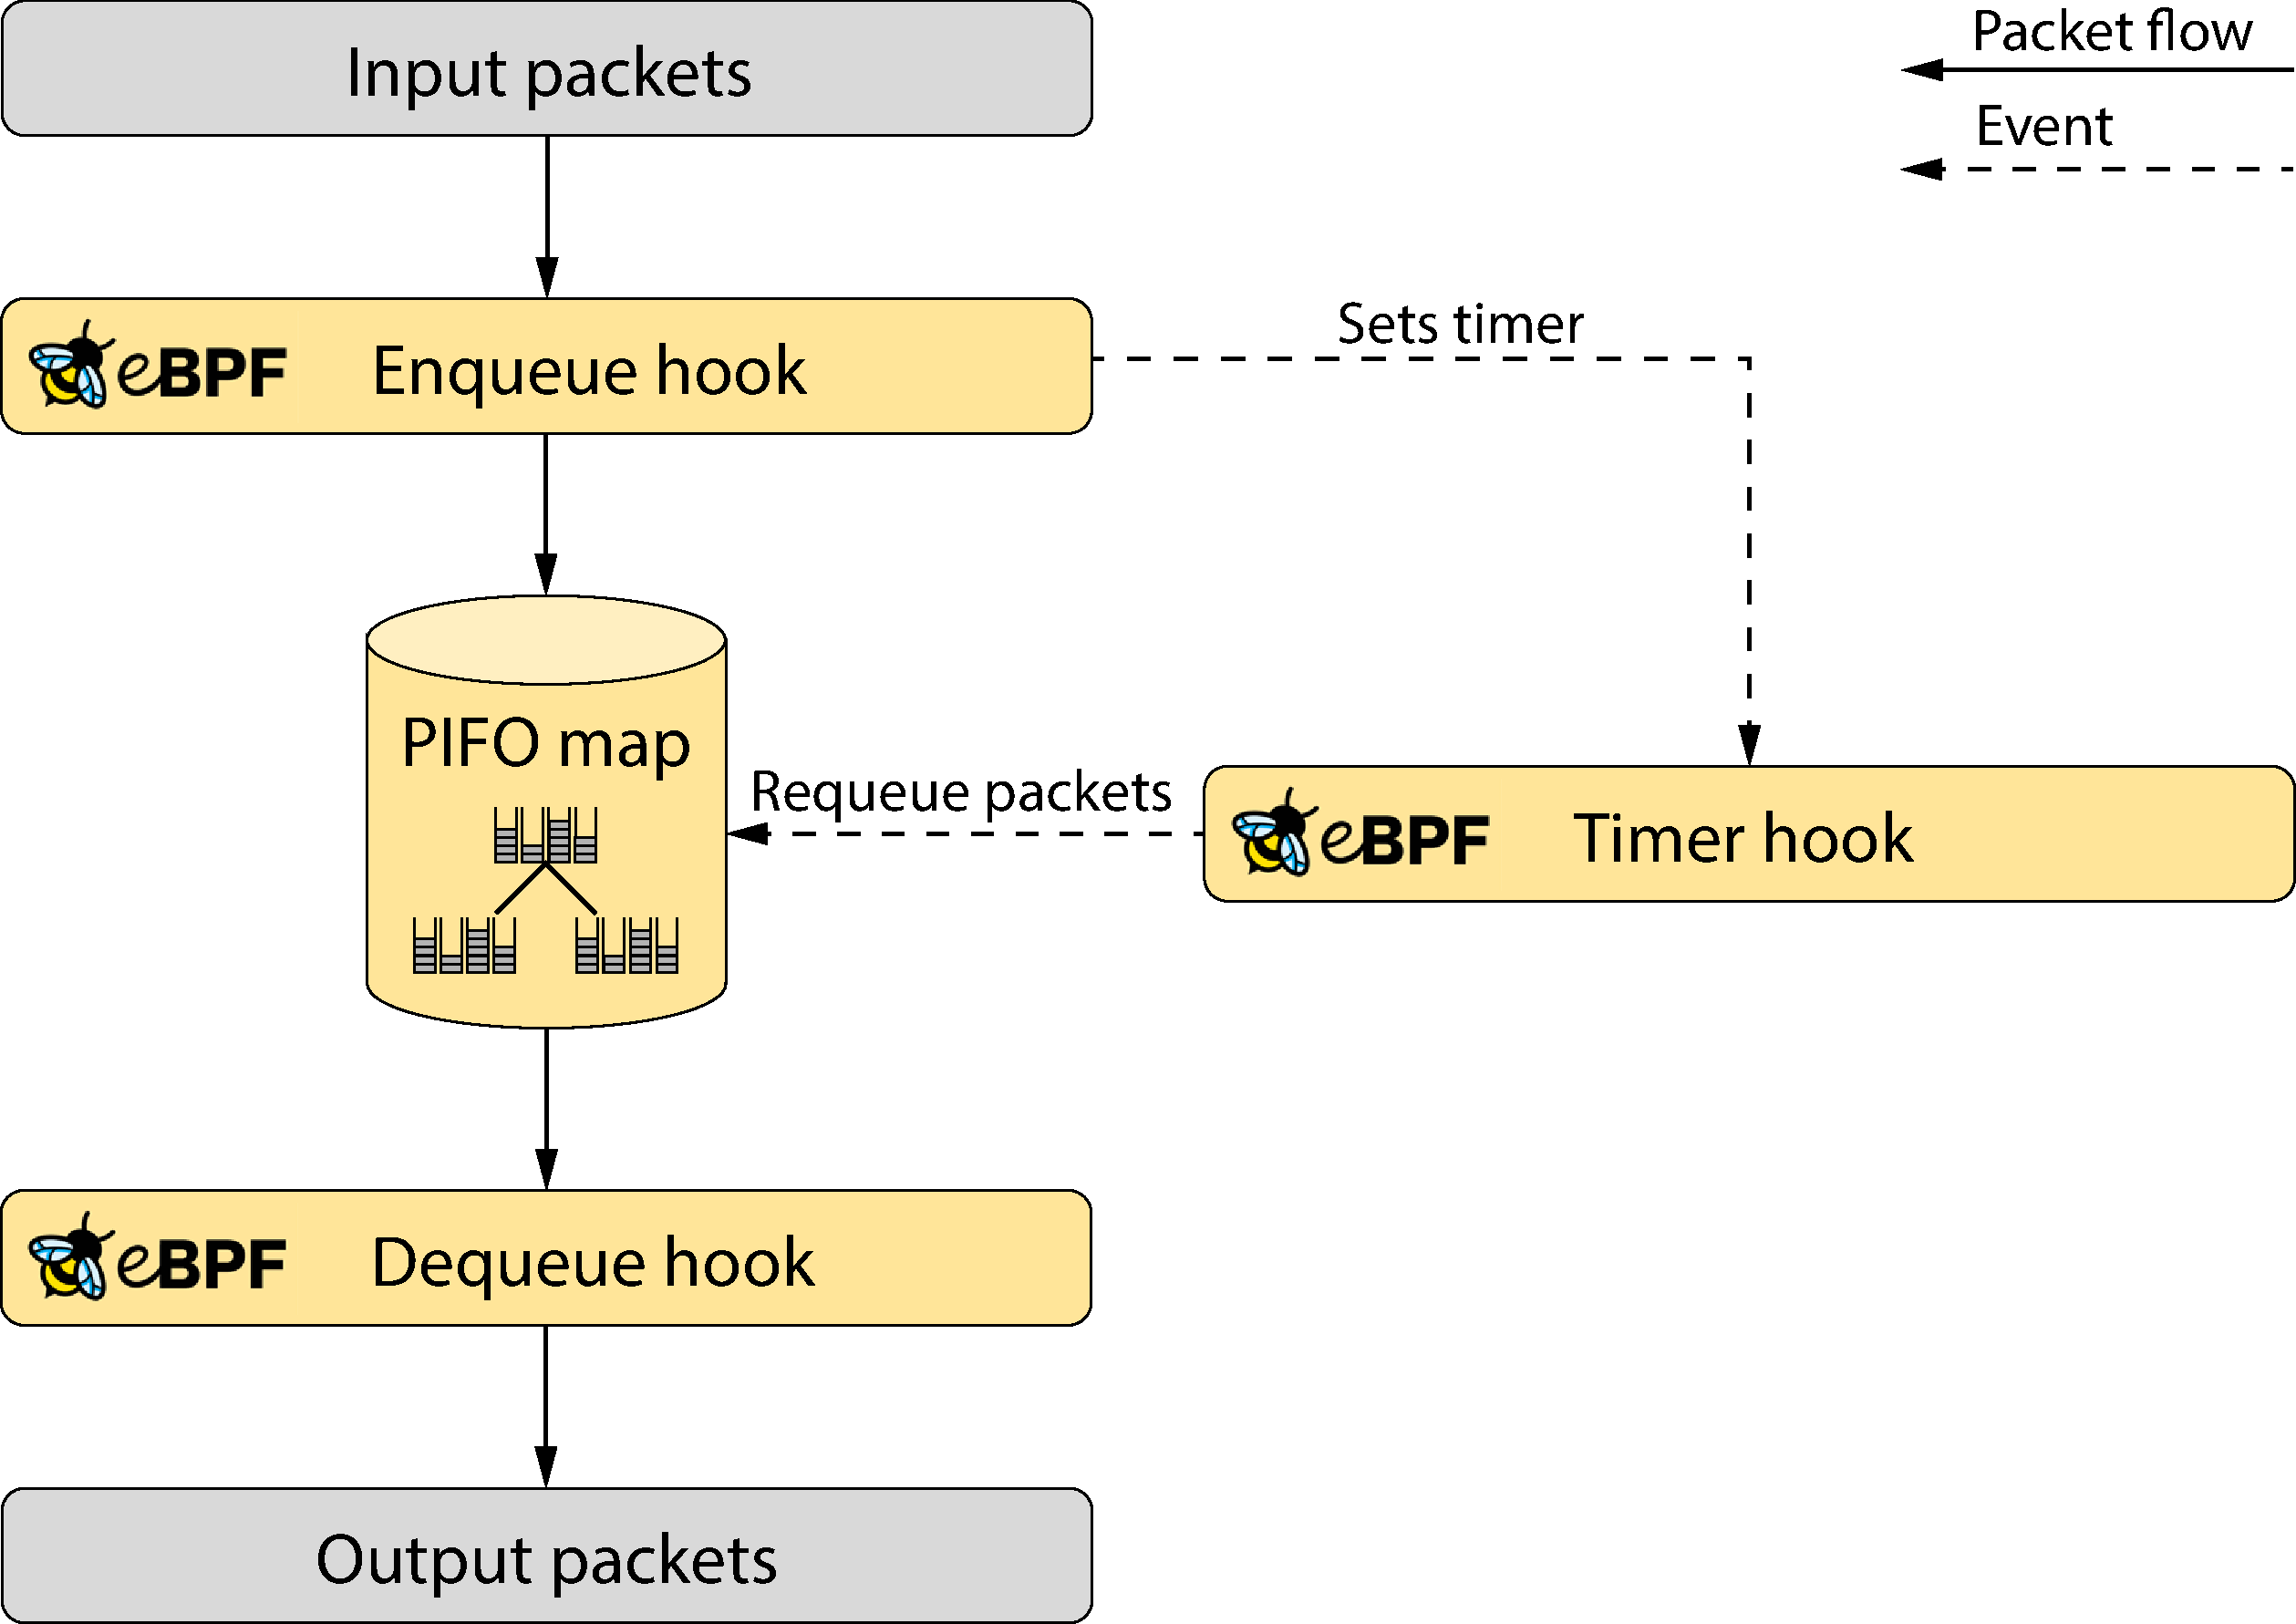
\includegraphics[width=\linewidth]{bpf_pps_flow.pdf}

  \caption{Depicted are the BPF hooks needed to implement programmable packet scheduling using our new proposed framework. The main hooks are the enqueue and dequeue hooks, with the optional timer hook. Queueing works the same in both XDP and the Qdisc. However, they do not use the same enqueue and dequeue hooks.\label{fig:bpf_pps_flow}}

\end{figure}

Our vision is to create an BPF based programmable packet scheduling framework that is flexible enough to share between the XDP and kernel Qdisc layers. The design is depicted in Figure \ref{fig:bpf_pps_flow}, which shows the basic building blocks for our design without the specifics of XDP nor the Qdisc subsystem.

These building blocks are then further broken down as follows:

\begin{itemize}
        \item Queue map: This new BPF map implements a PIFO and is the main building block for the programmer to create packet schedulers.
        \item Enqueue hook: This BPF hook is responsible for redirecting packets to BPF queue maps. This is the standard XDP hook in the case of XDP. However, it is a new hook in Qdiscs.
        \item Timer hook: This is an optional hook and is only required for algorithms that delay packets, e.g., packet pacing or traffic shaping. It is responsible for dequeuing and enqueuing packets from different PIFOs to introduce delayed packets. We implement timers using the newly introduced BPF timer API. This API allows the programmer to schedule BPF programs to be run at a specified time in the future, which can be used to release held packets.
        \item Dequeue hook: This hook is responsible for delivering the packet from the packet scheduling algorithm. In XDP, this is a new hook that each driver calls to transmit a packet. It can deliver bulking by repeatedly calling the hook to dequeue multiple packets before it transmits them.
\end{itemize}

Our design represents the PIFO data structure as an eBPF map. This representation allows the BPF programs to use a familiar map interface to reference PIFOs straightforwardly in their scheduling algorithm. From a programmer's perspective, the eBPF hooks reference the queues like any other map type. The enqueue hook can decide which queue to direct the packet to by a map reference. Similarly, the dequeue hook can pick which queue map to dequeue from and return a reference to the dequeued packet to the kernel for transmission. The BPF packet scheduling hooks can set BPF timers that trigger BPF programs at specified times if the scheduling algorithm needs to implement shaping and pacing. The BPF timer API supports both microsecond and nanosecond precision using the kernel's \textit{hrtimers}, making it ideal for our use case.


\section{BPF-Qdisc}

Due to XDP being only available in ingress and not at egress, queuing is only suitable for forwarded packets. However, if we want to support packets from the local machine, we provide a BPF-Qdisc that supports XDQ the same way as in XDP. To support this, we have created a new Qdisc that includes two separate hooks for ingress and egress to reflect our original design.


\section{eXpress Data Queueing (XDQ)}

Our design extends XDP by adding a new dequeue hook into the network drivers. We rely on standard XDP to enqueue packets into BPF queue maps. However, the new dequeue hook supports bulking by having the driver repeatedly dequeue packets from the dequeue hook before it transmits the packets.


\section{Evaluation of BPF-Qdisc and XDQ}

\begin{itemize}
  \item Compare a type of scheduling algorithm using BPF-Qdisc and XDQ performance to Qdiscs that does the same functionality.
  \item Compare BPF-Qdisc and XDQ performance to each other.
\end{itemize}

\section{Conclusion}

\begin{itemize}
  \item Reiterate main points of design, and summarize results.
\end{itemize}



\bibliographystyle{ACM-Reference-Format}
\bibliography{references}


\end{document}
\endinput
